%----------------------------------------------------------------------------------------
%	PACKAGES AND THEMES
%----------------------------------------------------------------------------------------
\documentclass[aspectratio=169,xcolor=dvipsnames]{beamer}
\usetheme{SimplePlus}

\usepackage{tikz}
\usetikzlibrary{arrows.meta,positioning}
\usepackage{listings}
\newsavebox{\longspecbox}
\lstset{basicstyle=\ttfamily\scriptsize,columns=fullflexible,keepspaces=true,showstringspaces=false,aboveskip=3pt,belowskip=3pt}

\usepackage{hyperref}
\usepackage{graphicx} % Allows including images
\usepackage{qrcode}
\usepackage{booktabs} % Allows the use of \toprule, \midrule and \bottomrule in tables

% Introduce each section with a roadmap highlighting the section ahead.
\AtBeginSection[]{%
    \begingroup
    \setbeamercolor{section in toc}{fg=DarkBlue}
    \setbeamercolor{section in toc shaded}{fg=black!30}
    \setbeamertemplate{section in toc shaded}[default][100]
    \begin{frame}{Roadmap}
        \tableofcontents[sectionstyle=show/shaded,subsectionstyle=show/show/hide]
    \end{frame}
    \endgroup
}

% Give each practice and lessons block a clear visual transition.
\AtBeginSubsection[]{%
    \begin{frame}
        \centering
        {\large\color{DarkBlue}\insertsectionhead\par}
        \vspace{0.8cm}
        {\Huge\bfseries\color{DarkBlue}\insertsubsectionhead\par}
    \end{frame}
}

%----------------------------------------------------------------------------------------
%	TITLE PAGE
%----------------------------------------------------------------------------------------

\title[AI Meets Formal Verification]{AI Meets Formal Verification: Practice and Prospects} % The short title appears at the bottom of every slide, the full title is only on the title page
% \subtitle{Subtitle}

\author[Pin-Yen] {Liao Zhang}

\institute[NTU] % Your institution as it will appear on the bottom of every slide, may be shorthand to save space
{
    Beneficial AI Foundation \\
}
% \date{\today} % Date, can be changed to a custom date
\date{November 6, 2026} % Date, can be changed to a custom date


%----------------------------------------------------------------------------------------
%	PRESENTATION SLIDES
%----------------------------------------------------------------------------------------

\begin{document}

\begin{frame}
    % Print the title page as the first slide
    \titlepage
\end{frame}

\begin{frame}{Overview}
    % Throughout your presentation, if you choose to use \section{} and \subsection{} commands, these will automatically be printed on this slide as an overview of your presentation
    \tableofcontents
\end{frame}

\begin{frame}{About Me}
    \begin{itemize}
        \item Research Scientist at the Beneficial AI Foundation.
        \item Working on AI for formal verification since 2018.
        \item PhD from the University of Innsbruck, Austria.
        \item Research focus: AI for mathematics and software development.
        % \item The first to use AI to generate explicit rules about how to apply tactics
        % \item The first to apply AI for term rewriting
        % \item Build the first comprehensive benchmark on property based testing for codeing agents
    \end{itemize}
\end{frame}

%------------------------------------------------
\begin{frame}{Selected Research}
    \begin{columns}[T,onlytextwidth]
        \begin{column}{0.48\textwidth}
            \begin{block}{AI for Term Rewriting}
                \small Pioneering AI methods for term rewriting, solving the most problems in the annual Confluence Competition.
            \end{block}
            \medskip
            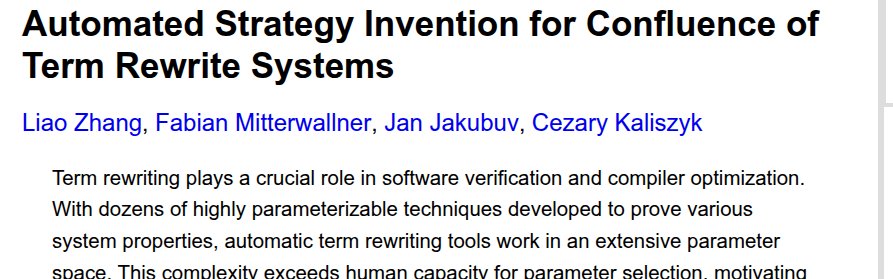
\includegraphics[width=\linewidth]{img/aaai.png}
        \end{column}
        \begin{column}{0.48\textwidth}
            \begin{block}{Interpretable Tactic Prediction}
                \small Learning explicit rules that explain tactic predictions in interactive theorem proving.
            \end{block}
            \medskip
            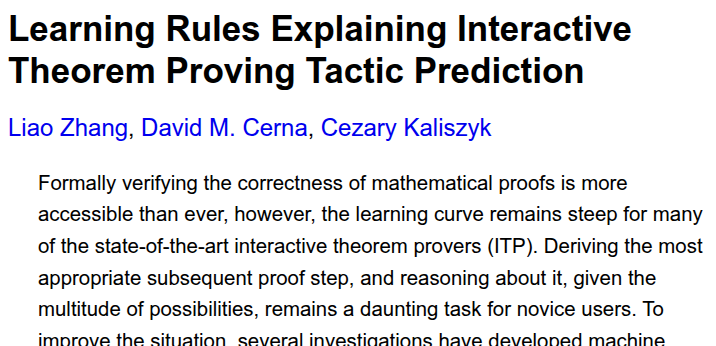
\includegraphics[width=\linewidth]{img/ijclr.png}
        \end{column}
    \end{columns}
\end{frame}

\begin{frame}{Selected Research}
    \begin{block}{Evaluating AI Agents on Property-Based Testing}
        \small From documentation to semantic invariants and input-generation strategies that reveal bugs.
    \end{block}
    \medskip
    \centering
    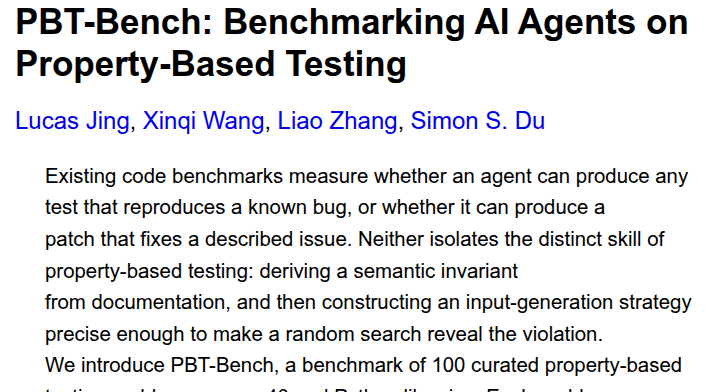
\includegraphics[width=0.78\textwidth,height=0.58\textheight,keepaspectratio]{img/pbt-bench.png}
\end{frame}

\section{Background: Beneficial AI Foundation and Signal Shot}
%------------------------------------------------

\begin{frame}{Beneficial AI Foundation}
    \begin{columns}[c,onlytextwidth]
    \begin{column}{0.70\textwidth}
    \small
    \begin{block}{Mission}
        Keep AI beneficial for humanity through technical AI safety research.
    \end{block}
    \begin{itemize}
        \item Founded by Max Tegmark.
        \item A central question: how can we make AI systems safer and more reliable?
        \item One approach: use AI to generate programs, formally verify their
              correctness and safety properties, and use the verified programs
              to carry out user tasks.
    \end{itemize}
    \medskip
    \footnotesize
    \textbf{Connection to practice:} cryptographic software provides concrete, demanding verification tasks.
    \end{column}
    \begin{column}{0.26\textwidth}
        \centering
        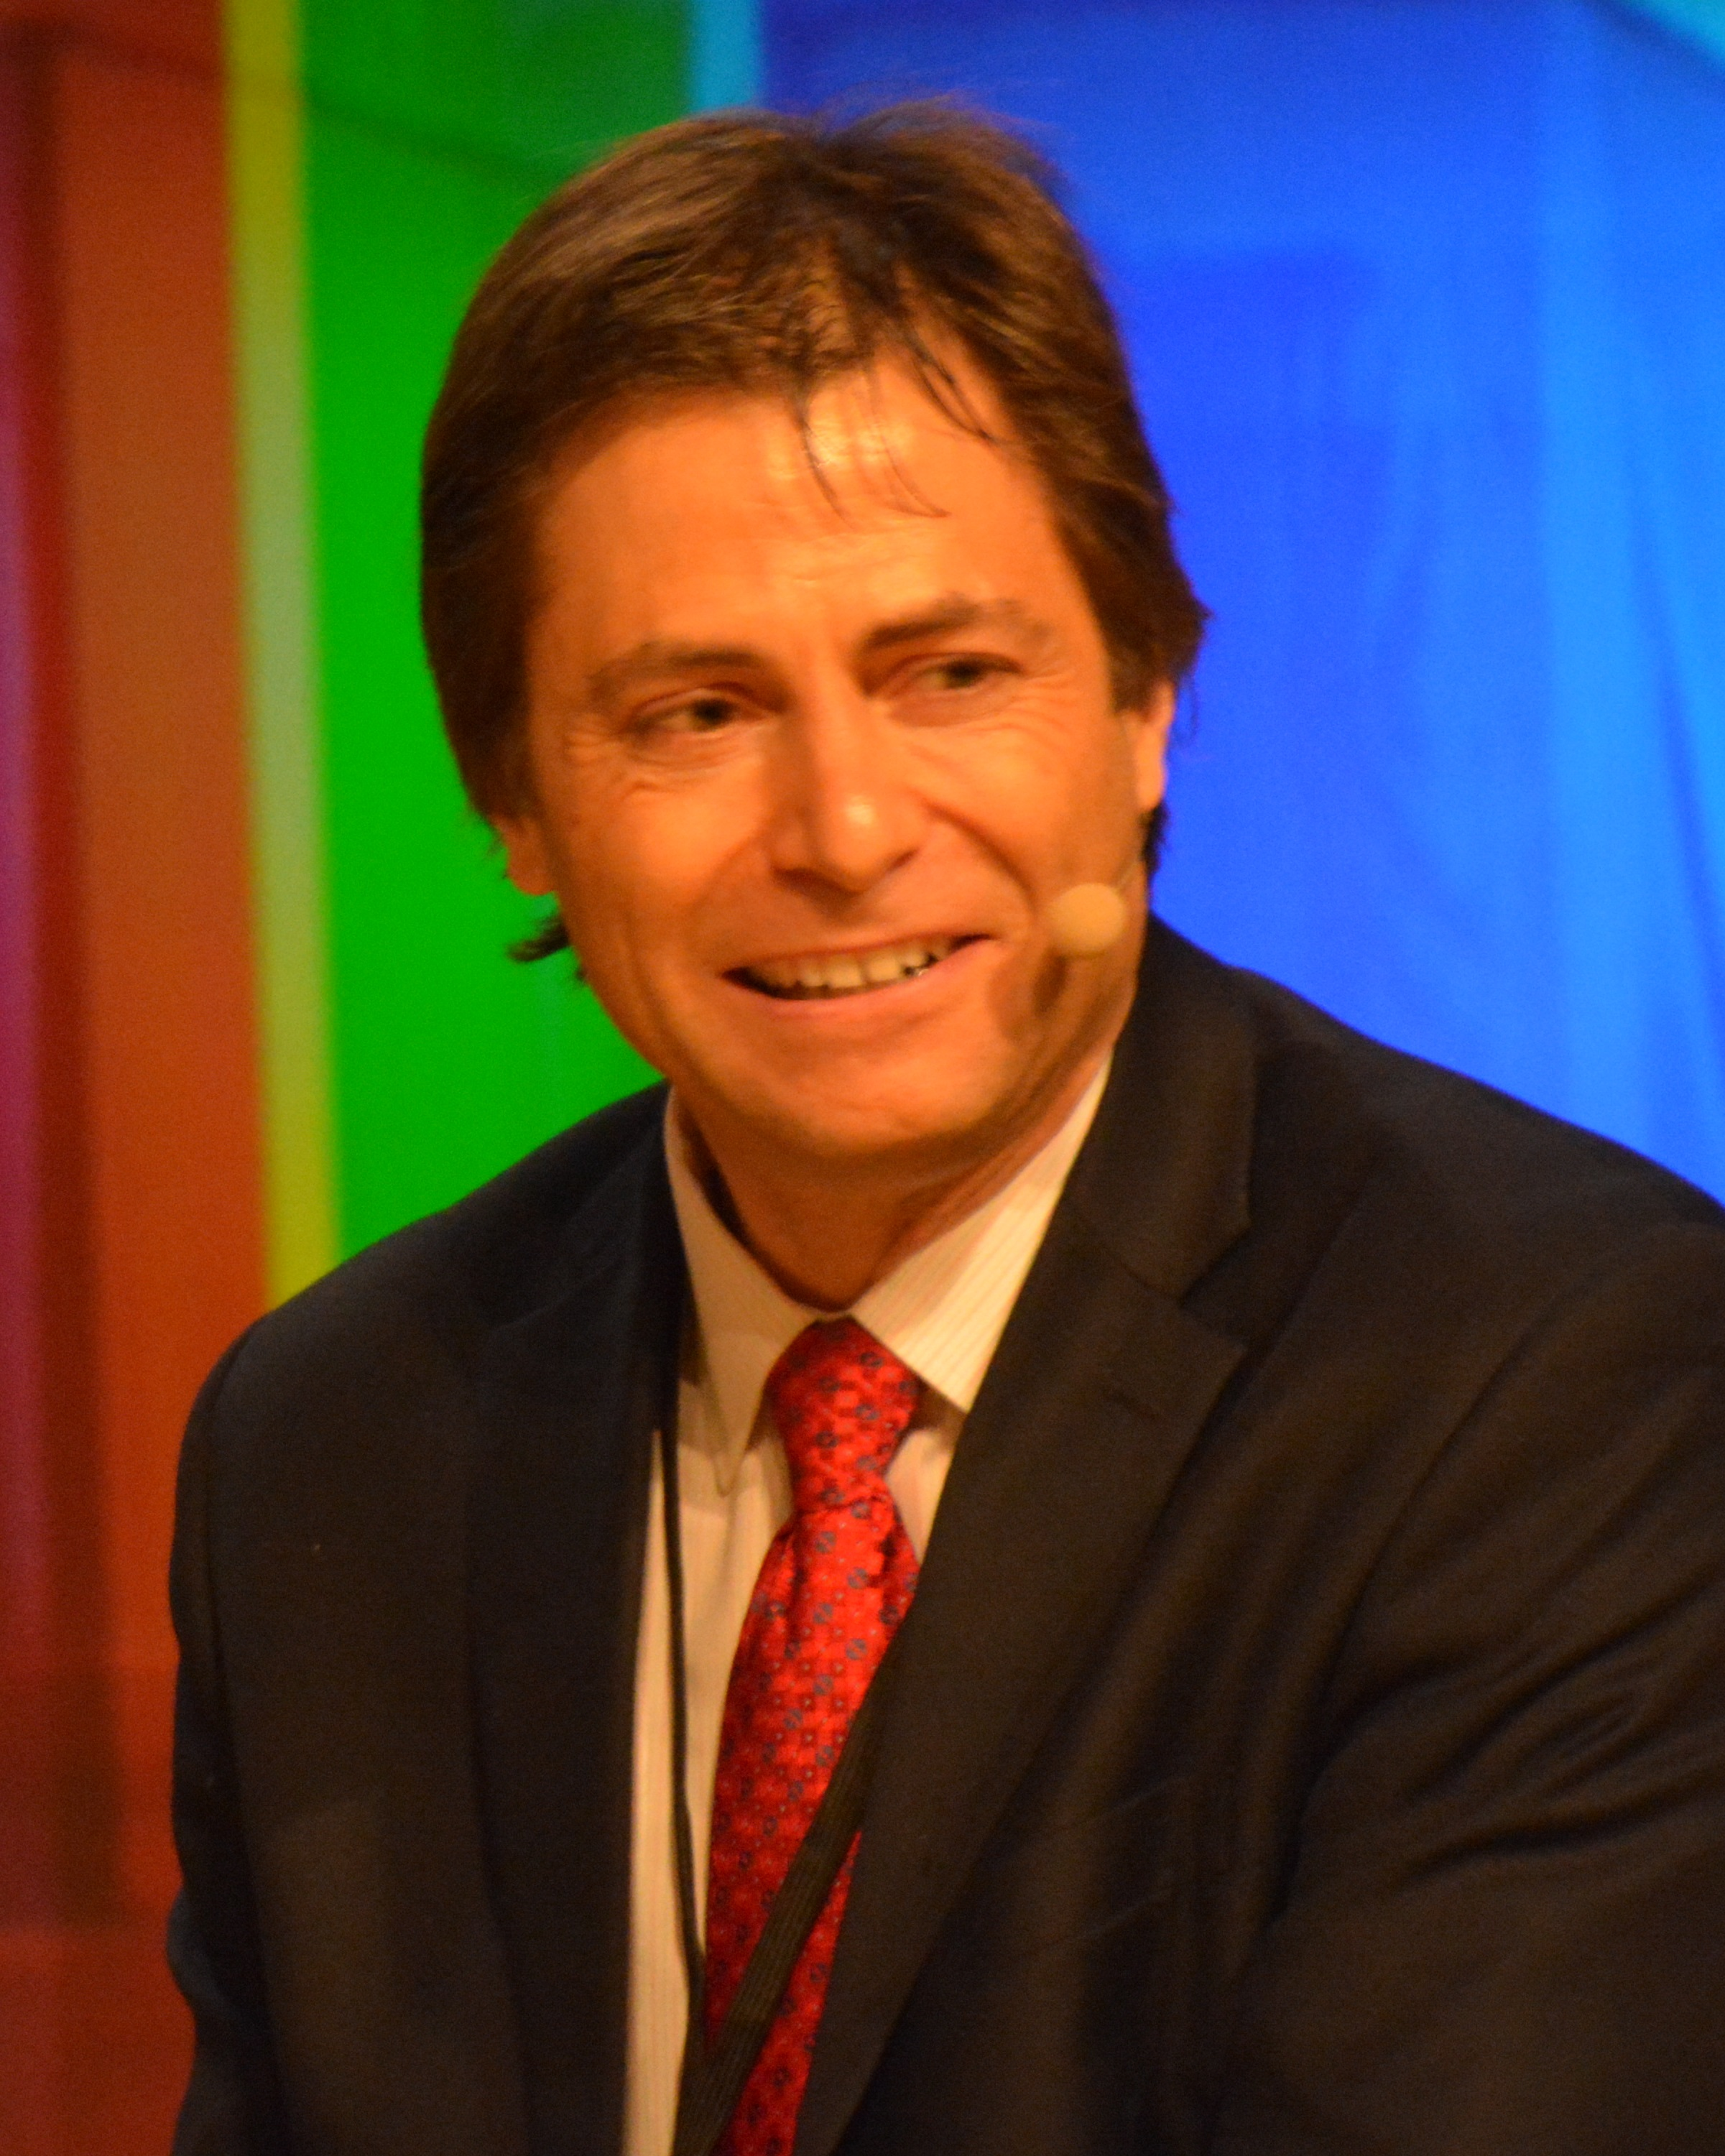
\includegraphics[width=\linewidth,height=3.8cm,keepaspectratio]{img/max-tegmark.jpg}
        \smallskip

        {\small\textbf{Max Tegmark}\par}
    \end{column}
    \end{columns}
\end{frame}

\begin{frame}{What Is Signal?}
    \small
    \begin{columns}[c,onlytextwidth]
    \begin{column}{0.74\textwidth}
    \begin{itemize}
        \item \textbf{Signal the app:} a messaging app for private conversations, including text messages, group chats, and voice/video calls.
        \item \textbf{End-to-end encryption:} messages are encrypted on the sender's device and decrypted on the recipient's device. The server relays ciphertext without access to the decryption keys.
        \item \textbf{Signal Protocol:} the cryptographic protocol underlying these encrypted conversations.
    \end{itemize}
    \end{column}
    \begin{column}{0.23\textwidth}
        \centering
        
\includegraphics[width=\linewidth]{img/signal.png}
    \end{column}
    \end{columns}
    % \begin{exampleblock}{Example: Alice Sends Bob a Message}
    %     Alice's device encrypts $\longrightarrow$ the server relays ciphertext
    %     $\longrightarrow$ Bob's device decrypts.
    % \end{exampleblock}
    \textbf{Why verification?} 
    % Security depends on both the protocol design and its software implementation behaving as intended.
    Establish that the protocol and its implementation satisfy their intended security properties.
    \medskip

\end{frame}

\begin{frame}{Signal Shot: A Shared Verification Challenge}
    \small
    \textbf{Launched in April 2026:} a collaborative initiative to formally verify
    the Signal protocol and application using Lean.
    \begin{itemize}
        \item \textbf{Technical ambition:} work toward machine-checked guarantees across the protocol stack and its implementation.
        \item \textbf{Engineering ambition:} develop reusable tools for protocol design and continuous verification as software changes.
        \item \textbf{Community ambition:} bring together Lean, cryptography, software verification, and AI-assisted theorem proving.
        \item \textbf{Concrete workstreams:} the initiative links verification repositories for libsignal, PQXDH, and SPQR.
    \end{itemize}
    % \begin{block}{From the Initiative to This Talk}
    %     SPQR is our practical case study: writing specifications, constructing Lean proofs,
    %     and understanding where AI helps and where human judgment remains essential.
    % \end{block}
\end{frame}

%------------------------------------------------
\section{SPQR and Dalek}
\subsection{Practice}
%------------------------------------------------


% Aeneas pipeline: https://aeneasverif.github.io/projects/
% Semantic foundation: https://arxiv.org/abs/2404.02680
% Functional translation: https://arxiv.org/abs/2206.07185
% Project overview: SparsePostQuantumRatchet-verify/README.md and src/lib.rs;
% src/incremental_mlkem768.rs; Spqr/Specs/Braid/Scka/EpochUniqueness.lean.
\begin{frame}{SPQR: A Key-Updating Component of Signal}
    \small
    \textbf{SPQR = Sparse Post-Quantum Ratchet}
    \begin{itemize}
        \item \textbf{The protocol:} a component of Signal that updates encryption keys during a conversation, designed to resist quantum attacks.
        \item \textbf{The code:} Signal also provides a Rust library implementing SPQR. This is the software we study.
        % \item \textbf{Why ``sparse''?} The data needed for a fresh post-quantum key update is spread across multiple messages.
    \end{itemize}
    \medskip
    \textbf{Intuition:} Alice and Bob keep updating their keys as they exchange messages.
    \begin{block}{What We Verify}
        Using Lean, we prove properties of the \textbf{Rust code}: for example,
        that data is encoded correctly and key-update steps follow their specifications.
        This is implementation correctness, not a proof of all of Signal's security.
    \end{block}
\end{frame}

\begin{frame}{SPQR: From Rust Code to Checked Proofs}
    \small
    \textbf{Target:} functional correctness of Signal's Sparse Post-Quantum Ratchet.
    \begin{center}
    \begin{tikzpicture}[
        stage/.style={draw=MediumBlue,fill=InvisibleBlue,rounded corners=3pt,
            text width=2.65cm,minimum height=0.75cm,align=center,inner sep=5pt,font=\small},
        flow/.style={-{Stealth[length=2mm]},thick,MediumBlue},
        node distance=0.65cm]
        \node[stage] (rust) {\textbf{Rust code}};
        \node[stage,right=of rust] (lean) {\textbf{Lean function}};
        \node[stage,right=of lean] (spec) {\textbf{Specification}};
        \node[stage,right=of spec] (proof) {\textbf{Checked proof}};
        \draw[flow] (rust) -- node[above,font=\scriptsize] {Aeneas} (lean);
        \draw[flow] (lean) -- (spec);
        \draw[flow] (spec) -- (proof);
    \end{tikzpicture}
    \end{center}

    \medskip
    \begin{enumerate}
        \item \textbf{Translate:} use Aeneas to turn the Rust implementation into Lean functions.
        \item \textbf{Specify:} state what those functions should do, including their assumptions.
        \item \textbf{Prove:} construct proofs that the translated functions satisfy these specifications; Lean checks the proofs.
    \end{enumerate}
    \medskip
    \begin{block}{The Key Distinction}
        Translation gives us code we can reason about in Lean.
        Specifications and proofs establish the properties we want to verify.
    \end{block}
\end{frame}

\begin{frame}{Aeneas: Translating Rust into Lean}
    \small
    \textbf{Inside the translation: Rust control flow becomes a functional model}
    \begin{center}
    \begin{tikzpicture}[
        ir/.style={draw=MediumBlue,fill=InvisibleGreen,rounded corners=3pt,
            text width=2.65cm,minimum height=1.2cm,align=center,inner sep=5pt,font=\footnotesize},
        flow/.style={-{Stealth[length=2mm]},thick,MediumBlue},
        node distance=0.65cm]
        \node[ir] (rust) {\textbf{Rust source}\\Borrowing and\\mutation};
        \node[ir,right=of rust] (mir) {\textbf{MIR}\\Compiler\\intermediate form};
        \node[ir,right=of mir] (llbc) {\textbf{LLBC}\\Structured IR\\with borrows};
        \node[ir,right=of llbc] (lean) {\textbf{Pure Lean model}\\Value updates;\\success or failure};
        \draw[flow] (rust) -- node[above,font=\scriptsize] {rustc} (mir);
        \draw[flow] (mir) -- node[above,font=\scriptsize] {Charon} (llbc);
        \draw[flow] (llbc) -- node[above,font=\scriptsize] {Aeneas} (lean);
    \end{tikzpicture}
    \end{center}
    \footnotesize
    \begin{itemize}
        % \item \textbf{Extraction:} Charon simplifies MIR to ULLBC, then reconstructs loops and branches into LLBC (Low-Level Borrow Calculus).
        \item \textbf{Translation:} Aeneas symbolically executes LLBC, tracking values, borrows, and loans. Mutation becomes explicit value updates in pure functions.
        \item \textbf{Semantic foundation:} formal results relate the borrow-based semantics to a heap-and-address model for the formalized language, not the entire Rust toolchain.
    \end{itemize}
\end{frame}

% Actual example: src/util.rs; SrcTranslated/Funs.lean (util.compare);
% Spqr/Specs/Util/Compare.lean. Translation excerpts shorten namespaces.
\begin{frame}[fragile]{SPQR Example: A Byte Comparison Loop}
    \lstset{basicstyle=\ttfamily\fontsize{7}{8}\selectfont}
    \small
    Compare two byte slices by accumulating differences with bitwise XOR and OR.
    \begin{columns}[T,onlytextwidth]
        \begin{column}{0.44\textwidth}
            \begin{block}{Rust: Mutation and a \texttt{for} Loop}
\begin{lstlisting}
fn compare(lhs: &[u8], rhs: &[u8]) -> u8 {
    let mut r: u8 = 0;
    for i in 0..lhs.len() {
        r |= lhs[i] ^ rhs[i];
    }
    is_non_zero(r)
}
\end{lstlisting}
            \end{block}
            \footnotesize
            \texttt{is\_non\_zero(r)} returns 0 if $r=0$, and 1 otherwise.
        \end{column}
        \begin{column}{0.53\textwidth}
            \begin{block}{Lean: Explicit State and \texttt{Result}}
\begin{lstlisting}[literate={←}{{$\leftarrow$}}1 {«}{{{\fontencoding{T1}\selectfont\guillemotleft}}}1 {»}{{{\fontencoding{T1}\selectfont\guillemotright}}}1]
def compare (lhs rhs : Slice U8) : Result U8 := do
  let n := Slice.len lhs
  let r ← compare_loop
    { start := 0#usize, «end» := n } lhs rhs 0#u8
  is_non_zero r
\end{lstlisting}
                \footnotesize Loop body at index \texttt{i} (names shortened):
\begin{lstlisting}[literate={←}{{$\leftarrow$}}1 {«}{{{\fontencoding{T1}\selectfont\guillemotleft}}}1 {»}{{{\fontencoding{T1}\selectfont\guillemotright}}}1]
let a ← Slice.index_usize lhs i
let b ← Slice.index_usize rhs i
let d ← lift (a ^^^ b)
let r1 ← lift (r ||| d)
ok (cont (iter1, r1))
\end{lstlisting}
            \end{block}
        \end{column}
    \end{columns}
    \footnotesize
    \begin{tabular}{@{}p{0.27\textwidth}p{0.68\textwidth}@{}}
        \textbf{Rust construct} & \textbf{Lean representation} \\\midrule
        \texttt{\&[u8]} & \texttt{Slice U8}: a borrowed byte slice becomes a value. \\
        \texttt{let mut r}; \texttt{for} & \texttt{loop} threads state \texttt{(iter, r)}; \texttt{cont} continues, \texttt{done} exits. \\
        \texttt{lhs[i]} & \texttt{Slice.index\_usize}: a checked access in \texttt{Result}; failure propagates. \\
    \end{tabular}
\end{frame}

\begin{frame}[fragile]{SPQR Example: Specification and Proof}
    \lstset{basicstyle=\ttfamily\fontsize{7}{8}\selectfont}
    \begin{block}{Specification and Top-Level Proof (\texttt{compare\_spec})}
\begin{lstlisting}[escapeinside={(*@}{@*)}]
theorem compare_spec (lhs rhs : Slice U8)
    (hlen : lhs.length = rhs.length) :
    compare lhs rhs (*@$\lbrace\!\lbrace$@*) (result : U8) =>
      result.val =
        if ((*@$\forall$@*) (j : Nat), j < lhs.length (*@$\to$@*) lhs.val[j]! = rhs.val[j]!)
        then 0 else 1 (*@$\rbrace\!\rbrace$@*) := by
  unfold compare
  step*
  grind
\end{lstlisting}
    \end{block}
    \footnotesize
    \textbf{Meaning:} equal-length inputs $\Rightarrow$ successful execution;
    return 0 for equal slices and 1 otherwise.
    \smallskip

    \textbf{Loop invariant:} $r=0\ \Longleftrightarrow\ \forall j<i,\;\mathit{lhs}[j]=\mathit{rhs}[j]$.
    \smallskip

    \begin{tabular}{@{}p{0.12\textwidth}p{0.83\textwidth}@{}}
        \textbf{Initialize} & $i=0$, $r=0$: the empty prefixes match. \\[3pt]
        \textbf{Preserve} & OR accumulates XOR differences; bit-vector lemmas establish the invariant at $i+1$. \\[3pt]
        \textbf{Finish} & $n-i$ decreases; equal lengths ensure valid accesses. At $i=n$, use \texttt{is\_non\_zero}. \\
    \end{tabular}
    \smallskip

    \scriptsize
    \texttt{step*} applies helper specifications; \texttt{grind} closes the logical goal.
    The theorem establishes functional behavior, not constant-time execution.
\end{frame}

% Actual declaration: Spqr/Specs/V1/Chunked/SendCt/HeaderReceived/SendCt1Chunk.lean:116--176.
% All hypotheses and postconditions retained; comments omitted; two namespaces abbreviated.
\begin{frame}[fragile]{SPQR: Reviewing Long Specifications}
    \small
    \textbf{\texttt{send\_ct1\_chunk\_spec}: 61 source lines before the proof begins.}\\
    {\scriptsize Complete statement below; comments omitted and namespaces shortened.}
    \begin{columns}[T,onlytextwidth]
        \begin{column}{0.49\textwidth}
\begin{lrbox}{\longspecbox}
\begin{minipage}{17cm}
\begin{lstlisting}[basicstyle=\ttfamily\fontsize{10}{10}\selectfont,escapeinside={(*@}{@*)},numbers=left,numberstyle=\tiny\color{gray},numbersep=3pt,firstnumber=1]
theorem send_ct1_chunk_spec {R : Type} (rngInst : rand_1.rng.Rng R)
    (cryptoInst : rand_core_1.CryptoRng R) (self : HeaderReceived) (rng : R)
    (h_hdr : self.uc.hdr.length = 64)
    (h_fill : (*@$\forall$@*) (r : R) (s : Slice U8),
      rngInst.rand_core_1RngCoreInst.fill_bytes r s (*@$\lbrace\!\lbrace$@*) fun _ => True (*@$\rbrace\!\rbrace$@*))
    (h_root : self.uc.auth.root_key.length + 32 (*@$\leq$@*) Usize.max) :
    send_ct1_chunk rngInst cryptoInst self rng (*@$\lbrace\!\lbrace$@*)
      (result : (v1.chunked.send_ct.Ct1Sampled (*@$\times$@*) encoding.Chunk (*@$\times$@*) EpochSecret) (*@$\times$@*) R) =>
      let st := result.1.1
      let chunk := result.1.2.1
      let es := result.1.2.2
      st.uc.epoch = self.uc.epoch (*@$\land$@*) st.uc.hdr = self.uc.hdr (*@$\land$@*)
      st.uc.ct1.length = 960 (*@$\land$@*) st.uc.es.length = F.encapsStateSize (*@$\land$@*)
      es.epoch = self.uc.epoch (*@$\land$@*) es.secret.length = 32 (*@$\land$@*)
      ((*@$\exists$@*) m : Fin 32 (*@$\to$@*) UInt8,
        st.uc.ct1.val = F.ct1List self.uc.hdr.val (by scalar_tac) m (*@$\land$@*)
        st.uc.es.val = F.toU8List
          (F.stateOut self.uc.hdr.val (by scalar_tac) m) (*@$\land$@*)
        es.secret.val = hkdf (replicate 32 0#u8)
          (F.toU8List
            (F.ssOut self.uc.hdr.val (by scalar_tac) m))
          (sckaKeyLabel ++ to_be_bytes self.uc.epoch) 32) (*@$\land$@*)
      st.uc.auth.root_key.length = 32 (*@$\land$@*) st.uc.auth.mac_key.length = 32 (*@$\land$@*)
      st.uc.auth.root_key.val ++ st.uc.auth.mac_key.val
        = hkdf (replicate 32 0#u8) (self.uc.auth.root_key.val ++ es.secret.val)
          (authenticator.Authenticator.updateLabel ++ to_be_bytes self.uc.epoch) 64 (*@$\land$@*)
      st.receiving_ek = self.receiving_ek (*@$\land$@*)
\end{lstlisting}
\end{minipage}
\end{lrbox}
\resizebox{\linewidth}{!}{\usebox{\longspecbox}}
        \end{column}
        \begin{column}{0.49\textwidth}
\begin{lrbox}{\longspecbox}
\begin{minipage}{17cm}
\begin{lstlisting}[basicstyle=\ttfamily\fontsize{10}{10}\selectfont,escapeinside={(*@}{@*)},numbers=left,numberstyle=\tiny\color{gray},numbersep=3pt,firstnumber=28]
chunk.index.val = 0 (*@$\land$@*)
chunk.data.length = 32 (*@$\land$@*)
st.sending_ct1.idx.val = 1 (*@$\land$@*)
((*@$\exists$@*) pts : Array Point 16#usize,
  ((*@$\forall$@*) (j : Nat), j < 16 (*@$\to$@*) (pts[j]!).value.length = 30) (*@$\land$@*)
  ((*@$\forall$@*) (j : Nat), j < 16 (*@$\to$@*) (*@$\forall$@*) (k : Nat), k < 30 (*@$\to$@*)
    (listToGF216Poly (pts[j]!).value).coeff k =
      (256 * st.uc.ct1.val[2 * (j + 16 * k)]! +
        (st.uc.ct1.val[2 * (j + 16 * k) + 1]!).val).toGF216) (*@$\land$@*)
  ((st.sending_ct1.s = .Points pts (*@$\land$@*)
    (*@$\forall$@*) (j : Nat), j < 16 (*@$\to$@*)
      PolyEncoder.chunkWord chunk.data j =
        ((pts[j]!).value[0]!).toGF216) (*@$\lor$@*)
   ((*@$\exists$@*) polys', st.sending_ct1.s = .Polys polys' (*@$\land$@*)
    ((*@$\forall$@*) (j : Nat), j < 16 (*@$\to$@*)
      polys'[j]!.toGF216Poly =
        (*@$\sum$@*) k (*@$\in$@*) Finset.range (pts[j]!).value.length,
          C (((pts[j]!).value[k]!).toGF216) *
            scaledLagrangeBasis (Vec.len ((pts[j]!).value)) k) (*@$\land$@*)
    ((*@$\forall$@*) (j : Nat), j < 16 (*@$\to$@*)
      (polys'[j]!).coefficients.length + 1 (*@$\leq$@*) Usize.max) (*@$\land$@*)
    ((*@$\forall$@*) (j : Nat), j < 16 (*@$\to$@*)
      PolyEncoder.chunkWord chunk.data j =
          ((pts[j]!).value[0]!).toGF216 (*@$\lor$@*)
      PolyEncoder.chunkWord chunk.data j =
        (polys'[j]!).toGF216Poly.eval (Nat.toGF216 0))))) (*@$\rbrace\!\rbrace$@*)
\end{lstlisting}
\end{minipage}
\end{lrbox}
\resizebox{\linewidth}{!}{\usebox{\longspecbox}}
        \end{column}
    \end{columns}
    \smallskip
    \footnotesize
    \textbf{Review:} shared randomness, HKDF labels, state preservation, byte indices, encoder branches.\\[3pt]
    \textbf{A checked proof does not tell us whether these are the right requirements.}
\end{frame}

\begin{frame}{SPQR: What Does This Specification Mean?}
    \small
    \textbf{Task:} generate the first ciphertext chunk after receiving a header.\\
    {\footnotesize Assumptions: a 64-byte header, successful RNG calls, and no key-length overflow.}
    \begin{center}
    \begin{tikzpicture}[
        box/.style={draw=MediumBlue,rounded corners=3pt,align=center,
            minimum height=1.05cm,inner sep=4pt,font=\footnotesize},
        flow/.style={-{Stealth[length=2mm]},thick,MediumBlue}]
        \node[box,fill=InvisibleBlue,text width=2.4cm] (input) at (0,0)
            {\textbf{Received header}\\Current epoch\\and root key};
        \node[box,fill=InvisibleGreen,text width=2.7cm] (encaps) at (3.5,0)
            {\textbf{Encapsulation}\\960-byte ciphertext\\and shared secret};
        \node[box,fill=InvisibleGreen,text width=2.7cm] (encode) at (7.1,0)
            {\textbf{Polynomial encoding}\\16 groups of\\30 two-byte values};
        \node[box,fill=InvisibleBlue,text width=2.4cm] (chunk) at (10.6,0)
            {\textbf{First chunk}\\Index 0\\32 data bytes};
        \draw[flow] (input) -- (encaps);
        \draw[flow] (encaps) -- (encode);
        \draw[flow] (encode) -- (chunk);
        \node[box,fill=InvisibleGreen,text width=4.4cm] (keys) at (3.5,-1.85)
            {\textbf{Derive and update keys}\\32-byte epoch secret via HKDF\\New root key and MAC key};
        \node[box,fill=InvisibleBlue,text width=4.4cm] (state) at (9,-1.85)
            {\textbf{State after the call}\\Next chunk index: 1\\Same epoch, header, and decoder};
        \draw[flow] (encaps) -- (keys);
        \draw[flow] (chunk.south) -- (10.6,-1.0) -- (state.north);
    \end{tikzpicture}
    \end{center}
    \footnotesize
    \begin{itemize}
        \item \textbf{Consistency:} ciphertext, saved encapsulation state, and shared secret
              must come from the same 32-byte random input.
        \item \textbf{Encoding:} the chunk must match that ciphertext, whether the encoder
              uses stored points or interpolating polynomials.
    \end{itemize}
    \smallskip
    \textbf{Why review is hard:} every link in this diagram becomes a precise logical condition.
\end{frame}

\begin{frame}{SPQR: When Specifications Do Not Compose}
    \small
    \textbf{Main failure: inconsistent variable bounds across specifications.}
    \begin{block}{Initially: Specifications Hold in Isolation}
        Each specification is true under its own variable bounds,
        and its proof checks with those assumptions.
    \end{block}
    \begin{columns}[T,onlytextwidth]
        \begin{column}{0.48\textwidth}
            \begin{exampleblock}{Later: Compose the Specifications}
                A caller must establish the variable bounds required by the callee's
                specification before applying it.
            \end{exampleblock}
        \end{column}
        \begin{column}{0.48\textwidth}
            \begin{exampleblock}{Why the Composition Fails}
                The specifications use different bounds.
                The bounds available at the call site do not imply those required
                by the callee, so the proof cannot proceed.
            \end{exampleblock}
        \end{column}
    \end{columns}
    \medskip
    \textbf{Repair at scale:} revise and align variable bounds across many specifications,
    then repair their proofs and the dependent proofs.
    \medskip

    \footnotesize
    \textbf{Lesson:} locally true specifications need compatible bounds to compose.
\end{frame}

% Cargo.toml [package.metadata.charon], translation-patches/lib-state_pb.patch.
\begin{frame}{SPQR: Code Outside the Translation}
    \small
    \textbf{Example: serializing the ratchet state with Protobuf (\texttt{prost}).}
    The project's extraction patch records problems translating the generated \texttt{Message} implementations.
    \begin{center}
    \begin{tikzpicture}[
        stage/.style={draw=MediumBlue,fill=InvisibleBlue,rounded corners=3pt,
            text width=3.5cm,minimum height=1.05cm,align=center,inner sep=5pt,font=\footnotesize},
        flow/.style={-{Stealth[length=2mm]},thick,MediumBlue},node distance=0.8cm]
        \node[stage] (rust) {\textbf{Rust caller}\\Save / load ratchet state};
        \node[stage,right=of rust] (wrap) {\textbf{Wrapper functions}\\\texttt{encode\_state\_pb}\\\texttt{decode\_state\_pb}};
        \node[stage,right=of wrap,fill=InvisibleGreen] (external) {\textbf{Lean external interface}\\Opaque to extraction;\\modeled separately};
        \draw[flow] (rust) -- (wrap);
        \draw[flow] (wrap) -- (external);
    \end{tikzpicture}
    \end{center}
    \begin{itemize}
        \item The extraction patch routes calls through wrappers and marks them \texttt{opaque}.
        \item This lets the surrounding code be translated without translating the \texttt{prost} implementation.
        \item The extraction configuration also excludes platform-specific SIMD and some generated trait implementations.
    \end{itemize}
    \begin{block}{The Extra Verification Obligation}
        A proof about a handwritten Lean model still needs justification that the external Rust code behaves like that model.
    \end{block}
\end{frame}

% SrcTranslated/FunsExternal.lean: Vec default model and proof; names shortened below.
\begin{frame}[fragile]{SPQR: Modeling External Functions in Lean}
    \footnotesize
    \lstset{basicstyle=\ttfamily\fontsize{8}{9}\selectfont}
    \begin{block}{Route 1: Write a Lean Model and Prove Its Specification}
        Example from the external models: \texttt{Vec::default} (names shortened).
\begin{lstlisting}[escapeinside={(*@}{@*)}]
def vec_default (T : Type) : Result (alloc.vec.Vec T) :=
  ok (alloc.vec.Vec.new T)

theorem vec_default_spec (T : Type) :
    vec_default T (*@$\lbrace\!\lbrace$@*) v => v.val = [] (*@$\rbrace\!\rbrace$@*) := by
  simp [vec_default, alloc.vec.Vec.new]
\end{lstlisting}
        The spec is proved from a body. Matching that model to Rust remains an obligation.
    \end{block}
    \begin{block}{Route 2: Extend Translation Support}
        Improve Charon/Aeneas support for the unsupported Rust features, then translate
        the implementation and prove its specification from the translated body.
    \end{block}
    % \textbf{Current Protobuf interface:} \texttt{encode\_state\_pb} uses
    % \texttt{opaque + axiom}; its behavior is assumed, not proved from a Lean model.
\end{frame}

% SrcTranslated/FunsExternal.lean: libcrux_hmac.hmac_sha256_tag32_spec.
\begin{frame}[fragile]{SPQR: Reviewing External Assumptions}
    \footnotesize
    \begin{block}{An External Declaration Only Gives the Type}
\begin{lstlisting}
noncomputable opaque libcrux_hmac.hmac : ...
\end{lstlisting}
        \texttt{Result (Vec U8)} allows failure or any output length;
        it does not guarantee success or 32 bytes.
    \end{block}
    \begin{block}{An Axiom Supplies the Missing Contract}
\begin{lstlisting}
axiom libcrux_hmac.hmac_sha256_tag32_spec ...
\end{lstlisting}
        If key and data lengths are $\leq$ \texttt{u32::MAX}, the SHA-256 call
        requesting 32 bytes succeeds and returns 32 bytes.
        Caller proofs use this guarantee. (Signatures shortened.)
    \end{block}
    \textbf{Why an axiom?} No translated implementation or Lean body is available
    to prove this contract.\\[2pt]
    \textbf{Why do not we write a Lean model:} sometimes proof is challenging and requires to write many definitions.
    We want faster progress. \\[2pt]
    \textbf{Review is challenging} 
\end{frame}

\begin{frame}{Dalek: What It Does and What We Verify}
    \small
    \begin{itemize}
        \item \textbf{What is it?} \texttt{curve25519-dalek} is a Rust library for group operations on Curve25519 (Edwards and Montgomery forms) and Ristretto.
        \item \textbf{What does it compute?} Point addition $P+Q$, scalar multiplication $[s]P$, and conversions between points, scalars, and bytes.
        \item \textbf{Where is it used?} These operations support key agreement, digital signatures, and zero-knowledge proofs; protocol libraries build on them.
    \end{itemize}
    \begin{block}{Our Verification Project}
        Use Aeneas and Lean to verify selected functions in the 64-bit serial backend:
        field arithmetic modulo $2^{255}-19$, byte encodings, and curve operations.
    \end{block}
    \footnotesize
    \textbf{Example guarantee:} for a valid point $P$ and scalar bytes with the top bit clear,
    scalar multiplication succeeds and returns a valid point $Q$ with
    \[
        \operatorname{toPoint}(Q)
        = [\operatorname{decode}(s)]\operatorname{toPoint}(P).
    \]
    This connects the concrete Rust computation to the mathematical group operation.
\end{frame}


\subsection{Lessons}

% \begin{frame}{AI Is Now Highly Capable}
%     \begin{itemize}
%         \item AI capabilities in constructing Lean proofs have improved substantially.
%         \item Simple prompts appear sufficient in most cases.
%         \item The clarity of AI-generated explanations has become a key bottleneck.
%         % Ask the AI to simplify its explanations.
%     \end{itemize}
% \end{frame}

\begin{frame}{AI Is Now Highly Capable}
    \begin{itemize}
        \item A year ago, AI struggled with challenging proofs in my workflow.
        \item Proofs involving loop invariants were particularly difficult.
        \item In my recent projects, AI has completed every proof task I have attempted with it.
        \item These include Lean proofs exceeding 1,000 lines.
        \item Most AI-generated specifications I have reviewed have been correct.
    \end{itemize}
\end{frame}

\begin{frame}{Simple Prompts Often Suffice}
    \begin{itemize}
        % \item One year ago, Claude Code skills were developed to guide AI workflows.
        % \item These skills use Markdown documents to provide instructions to AI agents.
        \item \textbf{MCP (Model Context Protocol)} is an open standard for connecting
              AI applications to external tools and data.
        \item An MCP server exposes tools that an AI agent can discover and call,
              then returns their results to the agent.
        \item \textbf{Lean MCP integrations}, such as \texttt{lean-lsp-mcp},
              connect the agent to Lean's language server and search tools:
        \begin{itemize}
            \item Inspect the current proof goal and local hypotheses.
            \item Read compiler errors, warnings, types, and documentation.
            \item Search for relevant lemmas and definitions.
            \item Try tactics or code snippets and inspect Lean's feedback.
        \end{itemize}
        \item \textbf{Workflow:} inspect a goal $\to$ propose a proof step
              $\to$ check with Lean $\to$ revise using feedback.
    \end{itemize}
\end{frame}

\begin{frame}{Simple Prompts Often Suffice}
    \begin{itemize}
        \item Recent improvements in AI capabilities have simplified my proof workflow.
        \item I examined Claude Code's behavior during Lean proof development.
        \item In the sessions I examined, it used neither skills nor MCP tools to construct Lean proofs.
        \item Direct file access and compilation were sufficient in these sessions.
        \item Structured proof views can help inspect individual goals.
        \item I also need project-wide information, such as the number of remaining \texttt{sorry} placeholders.
        \item In this workflow, elaborate prompts have offered limited additional benefit.
        \item My most useful instruction: ``Decompose the proof and compile after each completed step.''
        % \item Claude Code skills appear less useful in this workflow than they once were.
    \end{itemize}
\end{frame}


% https://www.anthropic.com/research/formalizing-fermats-last-theorem
% https://github.com/prove2me/prove2me_workspace/blob/main/references/prove.md
\begin{frame}{Example: Prove2Me and Fermat's Last Theorem}
    \begin{itemize}
        \item \textbf{Prove2Me} supported the Claude-agent project that formalized
              Fermat's Last Theorem in Lean.
        \item Agents can communicate with the remote platform through ordinary
              \textbf{HTTP requests and JSON responses}, using tools such as \texttt{curl}.
        \item Write and compile a proof locally, submit it for remote checking,
              then use the returned verdict and errors to revise it.
    \end{itemize}
    \begin{block}{A Simple Remote Verification Loop}
        \small
        \texttt{POST /api/v1/verify}: upload \texttt{solution.lean}; receive a submission ID.\\[5pt]
        \texttt{GET /api/v1/verify?submission\_id=...}: poll for the verdict and errors.
    \end{block}
    \begin{itemize}
        \item The platform tracks subtheorem dependencies so agents can work
              on separate parts of a large proof.
        \item \textbf{Takeaway:} a simple request--response interface can connect
              capable agents to a large-scale formal verification workflow.
    \end{itemize}
\end{frame}

\begin{frame}{Cross-Model Review for Specification Writing}
\begin{itemize}
\item AI can generate specifications, but these specifications may contain errors.

\item Complement manual review with independent reviews by different AI models.
\item This approach is particularly useful for less critical specifications.
\item Examples include helper lemmas and functions outside the public API.
\item In my experience, having different AI models independently check the same
      specification is highly effective at finding errors and omissions.
\end{itemize}

\end{frame}

\begin{frame}{Clarity of AI-Generated Explanations}
    \begin{itemize}
        \item Despite its capabilities, AI still requires human guidance.
        \item Clear, comprehensible explanations are essential for effective human oversight.
        \item AI systems tend to produce lengthy responses.
        \item My most frequent instruction is: ``Please shorten your response while preserving precision and clarity.''
        \item AI models should communicate their results in language that users can readily understand.
    \end{itemize}
\end{frame}

\section{Auto-Specifying Dalek}
\subsection{Practice}

% Based on auto_verify_dalek/docs/METHOD.md and
% harness/prove_top_spec.py / harness/dynamic_proof.py.
% Illustrative dependency chain, not a claim that this target is completed.
\begin{frame}{Auto-Specifying Dalek: Bottom-Up Proofs}
    \small
    \textbf{1. A human defines the public API specification, which remains fixed.}\\
    The implementation remains unchanged; AI writes internal specifications and proofs.
    \begin{center}
    \begin{tikzpicture}[
        contract/.style={draw=MediumBlue,rounded corners=3pt,align=center,
            minimum height=0.7cm,inner sep=5pt,font=\footnotesize},
        flow/.style={-{Stealth[length=2.5mm]},thick,MediumBlue}]
        \node[contract,fill=InvisibleBlue,text width=7.2cm] (api) at (0,0)
            {\textbf{4. Prove the fixed public API specification}\\
             \texttt{Scalar.invert\_spec} \quad (human-written statement)};
        \node[contract,fill=InvisibleGreen,text width=7.2cm] (internal) at (0,-1.2)
            {\textbf{3. AI specifies and proves the internal caller}\\
             \texttt{Scalar52.invert\_spec}};
        \node[contract,fill=InvisibleGreen,text width=3.4cm] (mul) at (-4.2,-2.4)
            {\texttt{montgomery\_mul\_spec}};
        \node[contract,fill=InvisibleGreen,text width=3.4cm] (to) at (0,-2.4)
            {\texttt{as\_montgomery\_spec}};
        \node[contract,fill=InvisibleGreen,text width=3.4cm] (from) at (4.2,-2.4)
            {\texttt{from\_montgomery\_spec}};
        \draw[flow] (mul.north) -- (internal.south west);
        \draw[flow] (to.north) -- (internal.south);
        \draw[flow] (from.north) -- (internal.south east);
        \draw[flow] (internal.north) -- (api.south);
        \node[font=\small,align=center] at (0,-3.15)
            {\textbf{2. AI writes and proves lower-level specs} (\texttt{Scalar52} helpers)};
    \end{tikzpicture}
    \end{center}
    \footnotesize
    \textbf{Arrows:} proved dependencies support the caller above; continue from the leaves to the API.\\
    \textbf{Feedback:} if an internal spec is too weak, revise it and recheck affected proofs.\\
    \textbf{Final check:} Lean proofs and project checks pass; the supplied API statement remains unchanged.
\end{frame}

% Conceptual round design requested for this talk: fresh context every round.
% Current harness/driver.py also supports resumed rounds and conditional resets;
% dynamic_proof.py implements dependency-ready scheduling in the harness.
\begin{frame}{Harness: Node Selection and Fresh Rounds}
    \small
    \textbf{Main agent:} decide which proof nodes to work on using the dependency graph.
    \begin{center}
    \begin{tikzpicture}[
        stage/.style={draw=MediumBlue,rounded corners=3pt,align=center,
            text width=3.45cm,minimum height=1.2cm,inner sep=5pt,font=\footnotesize},
        flow/.style={-{Stealth[length=2.5mm]},thick,MediumBlue}]
        \node[stage,fill=InvisibleBlue] (select) at (0,0)
            {\textbf{1. Select nodes}\\Read graph and summary;\\pick ready nodes};
        \node[stage,fill=InvisibleGreen] (work) at (4.6,0)
            {\textbf{2. Work on nodes}\\Write internal specs,\\lemmas, and proofs};
        \node[stage,fill=InvisibleGreen] (check) at (9.2,0)
            {\textbf{3. Check with Lean}\\Record checked results\\and remaining errors};
        \node[stage,fill=InvisibleBlue] (reset) at (0,-2.1)
            {\textbf{6. Start next round}\\Clear context;\\reload saved state};
        \node[stage,fill=InvisibleBlue] (save) at (4.6,-2.1)
            {\textbf{5. Save progress}\\Code, proof graph,\\summary, and diagnostics};
        \node[stage,fill=InvisibleBlue] (summary) at (9.2,-2.1)
            {\textbf{4. Write summary}\\Done / blocked / failed;\\next steps};
        \draw[flow] (select) -- (work);
        \draw[flow] (work) -- (check);
        \draw[flow] (check) -- (summary);
        \draw[flow] (summary) -- (save);
        \draw[flow] (save) -- (reset);
        \draw[flow] (reset) -- (select);
    \end{tikzpicture}
    \end{center}
    \begin{block}{Preserving Progress Across Sessions}
        \footnotesize
        Each round starts fresh, but retains the fixed API goal, code, dependency graph,
        and concise summaries. Repeat until the API proof and final checks pass.
    \end{block}
    \scriptsize
    Round design shown here: reset after every summary. The harness also supports session continuation.
\end{frame}

% Completed run documented in auto_verify_dalek/meet.md.
% Proof: ledger/transcripts/.proof-state-dag_scalar_invert_dynamic_01_32-8d43bea2-b4af-4a1c-809e-b828caf40bb0/
% round-1-draft/files/Curve25519Dalek/Specs/Scalar/Scalar/Invert.lean.
\begin{frame}[fragile]{Auto-Specifying Dalek: Scalar Inversion Proved}
    \small
    \textbf{Fixed API guarantee:} for input $x \not\equiv 0 \pmod{\ell}$,
    \texttt{Scalar.invert} succeeds and returns $y$ with $xy \equiv 1 \pmod{\ell}$.
    {\footnotesize Here $x,y$ decode the scalar bytes; $\ell$ is the scalar modulus.}
    \begin{columns}[T,onlytextwidth]
        \begin{column}{0.63\textwidth}
            \begin{block}{The Final Top-Level Proof}
\begin{lstlisting}[basicstyle=\ttfamily\fontsize{7}{8}\selectfont,escapeinside={(*@}{@*)}]
  unfold invert
  progress as (*@$\langle$@*)s, hs, hsb(*@$\rangle$@*)
  progress as (*@$\langle$@*)r, hrb, hrL, _hpow, hinv(*@$\rangle$@*)
  progress as (*@$\langle$@*)p, _hp1, hp(*@$\rangle$@*)
  have hL : _root_.L < 2 ^ 256 := by
    unfold _root_.L; norm_num
  rw [hp (by omega), (*@$\leftarrow$@*) hs]
  exact hinv (by rw [hs]; exact h)
\end{lstlisting}
            \end{block}
        \end{column}
        \begin{column}{0.34\textwidth}
            \begin{block}{What the Three Steps Use}
                \footnotesize
                \textbf{Unpack:} bytes to limbs.\\[4pt]
                \textbf{Invert:} apply the internal modular-inverse guarantee.\\[4pt]
                \textbf{Pack:} limbs back to bytes.
            \end{block}
        \end{column}
    \end{columns}
    \medskip
    \footnotesize
    \textbf{Completed run:} 31 proof nodes: 30 internal nodes + the fixed API spec.\\[3pt]
    \textbf{Validation:} original top-level statement preserved;
    no \texttt{sorry} dependencies in the final proof.
\end{frame}

% Illustrative checkpoint using the actual Scalar52.invert proof dependencies.
% Scheduling and gates: auto_verify_dalek/harness/dynamic_proof.py and driver.py.
\begin{frame}{Harness Example: Select a Node and Prove It}
    \footnotesize
    \textbf{Target:} \texttt{Scalar.invert\_spec}. Example checkpoint; selected dependencies shown.
    \begin{center}
    \begin{tabular}{@{}lll@{}}
        \toprule
        Node & Status & Scheduling decision \\
        \midrule
        \texttt{as\_montgomery\_spec} & Accepted & Reuse its guarantee \\
        \texttt{montgomery\_invert\_spec} & Accepted & Reuse its guarantee \\
        \texttt{from\_montgomery\_spec} & Accepted & Reuse its guarantee \\
        \texttt{Scalar52.invert\_spec} & Pending & \textbf{Ready: select this node} \\
        \texttt{Scalar.invert\_spec} & Pending & Wait for internal inversion \\
        \bottomrule
    \end{tabular}
    \end{center}
    \textbf{Selection rule:} choose a pending node only when all its dependencies are accepted.
    \begin{block}{Inside the Selected Node's Proof}
        \begin{enumerate}
            \item Specify limb bounds, $r<\ell$, and $r \equiv x^{\ell-2} \pmod{\ell}$.
            \item Unfold; use \texttt{progress} for the three accepted specs above.
            \item Prove the Montgomery round trip; for $x \not\equiv 0 \pmod{\ell}$,
                  use Fermat to derive $xr \equiv 1 \pmod{\ell}$.
        \end{enumerate}
    \end{block}
    \textbf{Check incrementally:} compile each helper, then the node; submit to the gate.
\end{frame}

\begin{frame}{Harness Example: What Makes the Gate Accept?}
    \footnotesize
    \textbf{Candidate:} the new \texttt{Scalar52.invert\_spec} and its helper proofs.
    \begin{center}
    \begin{tabular}{@{}p{0.20\textwidth}p{0.75\textwidth}@{}}
        \toprule
        Check & What the harness confirms \\
        \midrule
        Edit scope & Only permitted spec/helper files changed; implementation remains frozen. \\[2pt]
        Lean build & Definitions, statements, and proof terms check successfully. \\[2pt]
        Statement identity & Frozen declarations retain their fingerprints, including the supplied API spec. \\[2pt]
        Proof dependencies & No forbidden new axioms; no disallowed \texttt{sorryAx} in the theorem's transitive dependencies. \\
        \bottomrule
    \end{tabular}
    \end{center}
    \textbf{Example rejection:} a helper still contains \texttt{sorry}. Lean may compile the file,
    but the dependency check rejects the candidate if that helper is outside the allowed Math assumptions.
    \begin{block}{After All Checks Pass}
        Mark the node \texttt{accepted}, commit its proof, and save gate evidence in the graph.
        Once \texttt{unpack}, internal inversion, and \texttt{pack} are accepted,
        the public \texttt{Scalar.invert\_spec} becomes ready.
    \end{block}
    \textbf{Final gate:} publish only after every node and the final joint checks pass.\\[2pt]
    \textbf{For this successful run:} the final API proof has no \texttt{sorry} dependencies.
\end{frame}

\subsection{Lessons}

\begin{frame}{A Simple Harness Can Be Effective}
    \begin{itemize}
        \item Use a simple workflow to coordinate proof development.
        \item Assign a central agent to determine which proof node to expand next.
        \item Determine which proof nodes can be addressed within the current iteration.
        \item Record progress after each iteration.
        \item Reset the working context periodically, retaining concise progress summaries.
    \end{itemize}

\end{frame}

\begin{frame}{Decompose Proofs and Check Incrementally}
    \begin{itemize}
        \item Initial attempts to prove \texttt{to\_bytes} were unsuccessful.
        \item The \texttt{to\_bytes} implementation exceeds 700 lines of code, and proof attempts frequently time out.
        \item The key improvement was to decompose complex theorems into simpler lemmas.
        \item Make a small change, then check it with Lean.
        \item I think huge auto-formlaization project such as FLT can be completed like this.
    \end{itemize}
\end{frame}




%------------------------------------------------
\section{Prospects}
%------------------------------------------------

\begin{frame}{Future Directions for AI-Assisted Formal Verification}
    \begin{itemize}
        \item Efficient inference.
        \item Understandable formal verification.
    \end{itemize}
\end{frame}


\begin{frame}{Why Efficient Inference Matters}
    \begin{itemize}
        \item AI can now automate substantial parts of proof development and program verification.
        \item Long proof searches can require substantial token usage and computation.
        \item For practical adoption, verification costs must be justified by the value of the assurance gained.
        \item Reducing inference costs makes verification feasible for more software projects.
    \end{itemize}
\end{frame}

\begin{frame}{How to Improve Efficiency?}
    \small
    \begin{itemize}
        \item \textbf{Specialized small models and efficient inference}
        \begin{itemize}
            \item Vision already benefits from compact architectures, distillation,
                  pruning, and quantization.
            % MobileNets, Table 4: https://arxiv.org/abs/1704.04861
            \item \textbf{MobileNet:} 4,866M $\to$ 569M multiply-adds
                  (\textbf{88\% less computation}); ImageNet accuracy 71.7\% $\to$ 70.6\%.
            % LCM: https://arxiv.org/abs/2310.04378
            % \item \textbf{Image generation:} LCM distillation enables high-quality
            %       images in just \textbf{2--4 denoising steps}.
            % \item \textbf{Quantization:} FP32 $\to$ INT8 gives \textbf{4$\times$ smaller
            %       weight storage} before metadata; speed depends on hardware.
        \end{itemize}
        \item \textbf{Opportunity for math and code:} apply these ideas to specialized
              proof/code models; optimize \textbf{cost per verified solution}.
    \end{itemize}
\end{frame}

\begin{frame}{How to Improve Efficiency?}
    \begin{itemize}
        \item \textbf{Better verification frameworks}
        \begin{itemize}
            \item Decompose a goal into small subgoals.
            \item Let automated theorem provers solve routine subgoals.
            \item Improve the translation from Rust to Lean.
            \begin{itemize}
                \item Generate Lean functions that express Rust semantics clearly.
                \item Structure the translated code to simplify proof obligations.
            \end{itemize}
        \end{itemize}
    \end{itemize}
\end{frame}

\begin{frame}{Understandable Formal Verification}
    \begin{itemize}
        \item AI can generate proofs faster than people can read them.
        \item A checked proof still needs a clear explanation of its main ideas.
    \end{itemize}
    \medskip
    \centering
    {\small\textbf{Terence Tao, August 2026}\par}
    \smallskip
    \href{https://arxiv.org/abs/2608.16753}{
\includegraphics[width=0.55\textwidth]{img/tao-mathematics-ai-title.png}}
    \medskip

    \href{https://arxiv.org/pdf/2608.16753}{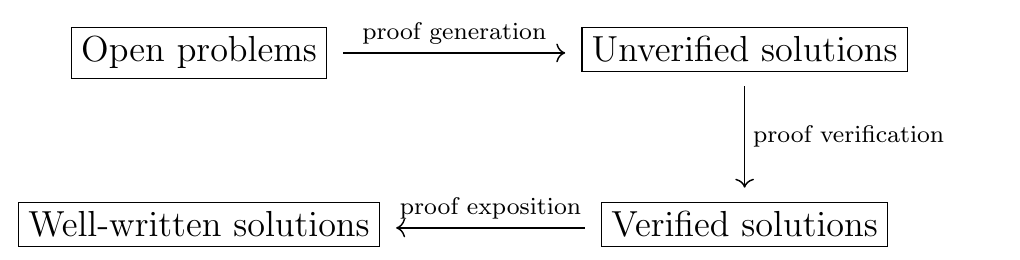
\includegraphics[width=0.70\textwidth]{img/tao-proof-exposition.png}}
    \smallskip

    {\small Proof explanations are essential for human understanding.\par}
\end{frame}


\begin{frame}{Understandable Formal Verification}
    \begin{itemize}
        \item Use proof assistants with \textbf{Controlled Natural Language (CNL)}.
        \item CNL resembles mathematical English, with restricted grammar
              and precise formal meaning.
        \item The system translates proof steps into logical obligations;
              automated provers check them.
    \end{itemize}
    \begin{block}{Illustrative CNL Sentences and Their Logical Meaning}
        \small
        \begin{tabular}{@{}ll@{}}
            Every prime number is greater than one.
                & $\forall p\in\mathbb{N},\;\mathrm{Prime}(p)\Rightarrow p>1$ \\
            There exists an even prime number.
                & $\exists p\in\mathbb{N},\;\mathrm{Prime}(p)\land\mathrm{Even}(p)$
        \end{tabular}
    \end{block}
    \begin{itemize}
        \item \textbf{Examples:} Naproche and Visored.
        \item \textbf{Key idea:} human-readable proofs with machine-checkable structure.
    \end{itemize}
\end{frame}
%------------------------------------------------

\begin{frame}
    \centering
    {\Huge\textbf{We Are Hiring}\par}
    \medskip
    {\large Beneficial AI Foundation\par}
    \bigskip
    \qrcode[height=3cm]{https://www.beneficialaifoundation.org/jobs}
    \bigskip

    {\small Scan to explore open positions\par}
    \medskip
    \href{https://www.beneficialaifoundation.org/jobs}{\footnotesize beneficialaifoundation.org/jobs}
\end{frame}

%----------------------------------------------------------------------------------------

\end{document}
